\input{preamble_ask.tex}
\input{definitions_ask.tex}



\pagestyle{askhseis}
\everymath{\displaystyle}

\begin{document}

\begin{center}
  \minibox{\large\bfseries \textcolor{Col1}{Επικαμπύλιο Ολοκλήρωμα ΙΙου είδους
  (Ανεξαρτησία Διαδρομής)}}
\end{center}

\vspace{\baselineskip}

\begin{enumerate}

% thomas ex 33 p. 931
  \item Για ποιές τιμές των $ a,b,c $ το διανυσματικό πεδίο $ \mathbf{F}(x,y,z) =
    (y^{2}+2czx)
    \,\mathbf{i} + y(bx+cz) \,\mathbf{j} + (y^{2}+cx^{2}) \,\mathbf{k} $ είναι 
    αστρόβιλο; \hfill Απ: $ a=1, \; b=2, \; c=2 $ 

  \item Για τα παρακάτω διανυσματικά πεδία αφού δείξετε με 2 τρόπους ότι είναι 
    αστρόβιλα (συντηρητικά), στη συνέχεια να βρεθεί η συνάρτηση δυναμικού.
    \begin{enumerate}[i)]
% thomas ex 7 p. 929
      \item $ \mathbf{F}(x,y,z) = 2x \mathbf{i} + 3y \mathbf{j} + 4z \mathbf{k}
        $ \hfill Απ: $ f(x,y,z) = x^{2}+ {3y^{2}}/{2} + 2z^{2} +c $ 
% thomas ex 8 p. 929
      \item $ \mathbf{F}(x,y,z) = (y+z) \mathbf{i} + (x+z) \mathbf{j} + (x+y) \mathbf{k}
        $ \hfill Απ: $ f(x,y,z) = (y+z)x+zy + c $ 
% thomas ex 10 p. 929
      \item $ \mathbf{F}(x,y,z) = (y \sin{z}) \mathbf{i} + (x \sin{z}) \mathbf{j} + (xy
        \cos{z}) \mathbf{k} $ \hfill Απ: $ xy \sin{z} + c $ 
    \end{enumerate}

% thomas ex 28 p. 930
  \item Αφού δείξετε ότι το διανυσματικό πεδίο $ \mathbf{F}(x,y,z) = (\mathrm{e}^{x}
    \ln{y}) \mathbf{i} +
    ({\mathrm{e}^{x}}/{y} + \sin{z}) \mathbf{j} + (y \cos{z}) \mathbf{k} $ 
    είναι συντηρητικό, στη συνέχεια να δείξετε ότι γράφεται ως κλίση κάποιας 
    πραγματικής συνάρτησης. \hfill Απ: $ \mathbf{F}= \grad (\mathrm{e}^{x} \ln{y} + y
    \sin{z}) $ 

  \item Να υπολογιστούν τα παρακάτω ολοκληρώματα αφού δείξετε ότι οι παραστάσεις της
    μορφής $ P dx + Q dy + R dz $ είναι τέλεια διαφορικά.
    \begin{enumerate}[i)]
% thomas ex 13 p. 930
      \item $ \int _{(1,1,2)}^{(3,5,0)} yz dx + xz dy + xy dz $ 
        \hfill Απ: $ -2 $ 
% thomas ex 13 p. 930
      \item $ \int _{(0,0,0)}^{(1,2,3)} 2xy dx + (x^{2}-z^{2}) dy -2yzdz $ 
        \hfill Απ: $ -16 $ 
% thomas ex 17 p. 930
      \item $ \int _{(1,0,0)}^{(0,1,1)} \sin{y} \cos{x} dx + \cos{y} \sin{x} dy + dz $ 
        \hfill Απ: $1$ 
    \end{enumerate}

  \item Να υπολογιστεί το έργο της $ \mathbf{F}(x,y,z) = (x^{2}+y) \mathbf{i} +
    (y^{2}+x) \mathbf{j} + (z \mathrm{e}^{z}) \mathbf{k} $ κατά μήκος της καμπύλης

    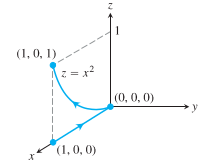
\includegraphics[scale=0.5]{int4.png}

    \hfill Απ: 1 

  \item Να υπολογιστεί το έργο της $ \mathbf{F}(x,y,z) = \mathrm{e}^{yz} \mathbf{i} +
    (xz \mathrm{e}^{yz} + z \cos{y}) \mathbf{j} + (xy \mathrm{e}^{yz} + \sin{y}) \mathbf{k} $ κατά μήκος της καμπύλης

    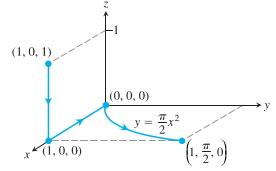
\includegraphics[scale=0.5]{int3.png}

    \hfill Απ: 0 
\end{enumerate}


\section*{Θεώρημα Green}


\begin{enumerate}
  %thomas exapmple 3 p. 937
  \item Να επαληθεύσετε και τις 2 εκδοχές του θεωρήματος Green για το διανυσματικό πεδίο 
    $ \mathbf{F}(x,y) = (x-y)\mathbf{i}+ x\mathbf{j} $ και για την επίπεδη περιοχή $D$ 
    που περικλείεται από την κλειστή και θετικά προσανατολισμένη καμπύλη 
    $ c \colon \mathbf{r}(t)= \cos{t}\, \mathbf{i} + \sin{t}\, \mathbf{j} $, με 
    $ 0 \leq t \leq 2 \pi $.

    \hfill Απ: $ \pi, \; 2 \pi  $ 

  \item Χρησιμοποιώντας το θεώρημα Green να υπολογίσετε την κυκλοφορία (αντιωρολογιακά) 
    και την εξερχόμενη ροή των παρακάτω διανυσματικών πεδίων: 
    \begin{enumerate}[i)]
  %thomas exapmple 6 p. 939
      \item $ \mathbf{F}(x,y) = (x^{2}+4y) \,\mathbf{i} + (x+y^{2}) \,\mathbf{j} $ 
        με $ c \colon $ τετράγωνο που γράφεται από $ x=0, x=1, y=0, y=1 $. 
        
        \hfill Απ: $ circ = -3, flux=2 $  
  %thomas exapmple 8 p. 939
      \item $ \mathbf{F}(x,y) = (x+y) \,\mathbf{i}- (x^{2}+y^{2}) \,\mathbf{j} $ 
        με $ c \colon $ τρίγωνο που γράφεται από $ y=0, x=1, y=x $.

        \hfill Απ: $ circ = -7/6, flux= 1/6$  
    \end{enumerate}

  \item Χρησιμοποιώντας το θεώρημα Green να υπολογίσετε την κυκλοφορία (αντιωρολογιακά) 
    και την εξερχόμενη ροή των παρακάτω διανυσματικών πεδίων: 
    \begin{enumerate}[i)]
  %thomas exapmple 9 p. 940
      \item $ \mathbf{F}(x,y) = (xy+y^{2}) \,\mathbf{i} + (x-y) \,\mathbf{j} $ 
        με $ c \colon $ την κλειστή καμπύλη που γράφεται από τις $ y=x^{2} $ και 
        $ x = y^{2} $.  

        \hfill Απ: $ circ = -7/60, flux= -11/60$  

  %thomas exapmple 11 p. 940
      \item $ \mathbf{F}(x,y) = (x^{3}y^{2}) \,\mathbf{i} + (1/2x^{4}y) \,\mathbf{j} $ 
        με $ c \colon $ την κλειστή καμπύλη που γράφεται από τις $ y=x $ και 
        $ y = x^{2}-x $.  

        \hfill Απ: $ circ = -7/60, flux= -11/60$  
    \end{enumerate}

    

    \section*{Πολλαπλά Συνεκτικό Χωρίο}

  \item Να υπολογιστεί το επικαμπύλιο ολοκλήρωμα $ \int _{c}
    \frac{ydx-xdy}{x^{2}+y^{2}} $, όπου $ c $ είναι περίμετρος τετραγώνου με κορυφές τα
    σημεία $(1,1), (-1,1), (-1,-1), (1,-1) $. \hfill Απ: $ -2 \pi $ 

  \item Να υπολογιστεί το επικαμπύλιο ολοκλήρωμα $ \int _{c}
    \frac{-ydx+xdy}{4x^{2}+9y^{2}} $, όπου $ c $ η καμπύλη $ x^{2}+y^{2}=16 $.
    \hfill Απ: $ \pi /3 $ 
\end{enumerate}





\end{document}

